\documentclass[conference]{IEEEtran}
\IEEEoverridecommandlockouts
% The preceding line is only needed to identify funding in the first footnote. If that is unneeded, please comment it out.
\usepackage{cite}
\usepackage{amsmath,amssymb,amsfonts}
\usepackage{algorithmic}
\usepackage{graphicx}
\usepackage{textcomp}
\usepackage{xcolor}
\def\BibTeX{{\rm B\kern-.05em{\sc i\kern-.025em b}\kern-.08em
    T\kern-.1667em\lower.7ex\hbox{E}\kern-.125emX}}
\begin{document}

\title{Term Project Part 1 Report\\
{\footnotesize CENG 435 Data Communications and Networking}
}

\author{\IEEEauthorblockN{Dogancan Kartal}
\IEEEauthorblockA{\textit{Department of Computer Engineering} \\
\textit{Middle East Technical University}\\
Ankara, Turkey \\
e2036028@ceng.metu.edu.tr}
\and
\IEEEauthorblockN{Mert Bekar}
\IEEEauthorblockA{\textit{Department of Computer Engineering} \\
\textit{Middle East Technical University}\\
Ankara, Turkey \\
e2035749@ceng.metu.edu.tr}
}

\maketitle

\begin{abstract}
This document is aimed to give the reader an intuition about our progress for the first part of the term project of CENG435 course.
\end{abstract}

\begin{IEEEkeywords}
Socket programming, UDP, TCP, Threading
\end{IEEEkeywords}

\section{Introduction}
In this project, we designed a network that consist of 5 nodes. A source node s, a broker b, two routers r1 and r2, and destination node d. We are tasked to send packets through the network and observe the experiments using several configurations. Packets are generated by source node and follows the path broker, one of the router and destination.2 A packet contains a trivial message content.

\section{Initial Setup}
We first created slice on GENI Portal. We are given an \textit{xml} file which consist of the information about the network topology. We added this \textit{xml} file to create the topology. We then picked the aggregate which will run our virtual machines. After this steps, we configured ssh and created version control repository. We used private GitHub repository for the entire development, upon request we can show the commit history. Then we were ready for implementation. 

\section{Topology}
We aimed to send the packets from source node to destination node through intermediate nodes. To handle this communication between nodes, we investigated the given network topology. We observed that nodes are connected by links. Each link has 2 interfaces, 1 interface for client 1 interface for server. We could achieve this aim by using the correct interfaces between nodes. For example, assume that we want to send a packet from source node to broker node, we handled this situation by sending the packet through broker interface of link between source node and broker node.

\section{Implementation}
After the initial configurations and the analyzing the topology, we started implementing. We used the Python programming language for this project.
\subsection{Introduction}
We first needed to create a packet in the source and send it to the broker node using TCP connection. When broker node receives the packet from the source node, broker node sends the packet to the one of the router nodes using UDP connection. The decision of which router to send is made randomly. When a router node receives the packet from broker node, it forwards the packet to the destination node using UDP connection. When destination node receives the packet from one of the router nodes, we immediately calculate the end-to-end delay and send back an acknowledgement. Acknowledgement follows the reversed path to the source node. \\
When we first started implementing, we did not think of returning an acknowledgement mechanism, but we did not get proper results to make the necessary experiments. Therefore, we used acknowledgement mechanism. More details will be discussed later.
\subsection{Source Node, \textbf{s}}
The main task of the source node is to generate and send the packets to the broker node with TCP connection. Initially, we created a socket object from socket module (default is TCP). Then, using \textit{connect} function with parameters host and port, we create a connection between source and broker nodes. The host parameter is obtained from the network topology. We checked the broker interface of the link between the source and broker nodes and used the IP address, ${10.10.1.2}$, as a host parameter. We selected the port 5000 of the broker's ports since we couldn't pick from the first 1024 ones. The number 5000 is totally random. \\
In order to obtain a valid distribution, we decided to generate 2000 packets. Each packet is a string of the creation time and its index. First 13 digits represent the creation time and last following 4 digits represent the index of that packet. For example; for the 100th packet, packet content is the following: $15435436096770100$. Then we added the keyword \textit{s} in order to see the path afterwards. After this operation, our packet content becomes $15435436096770100s$. Then, the packet is send to the broker node using TCP connection and the source node waits for the acknowledgement from broker node.
\subsection{Broker Node, \textbf{b}}
The main task of the broker node is to send the packets over multiple paths. The broker node is firstly a TCP server that receives data from source node with TCP. We have 2 possible routers to send the packets. We decided which router to send by using a \textit{randint} function from built-in \textit{random} module. After that step, we created a socket object from socket module with parameters \textit{socket.AF\textunderscore INET} and \textit{socket.SOCK\textunderscore DGRAM} in order to send a packet to the selected router. \\
Before sending the packet to the selected router, we first added the term $b$ to the received data in order to trace the path afterwards. So, for example; for the 100th packet that was received from the source node we send the data as $15435436096770100sb$. To conclude the broker node, it is both TCP server and UDP client for our network, it converts TCP streams to UDP datagrams and send those datagrams to one of routers. The broker node waits for the acknowledgement from the selected router node and after getting the acknowledgement, again appending the term $b$ to the received acknowledgement, we send it to the source node.
\subsection{Router Node i, \textbf{r_i}}
The main task of the router nodes are to send the packets to the destination node. The router nodes are firstly UDP servers that receive data from the broker node with UDP. Assume the broker node selected the 1st router node. It should bind the $r1$ interface of the intermediate link and it is $10.10.2.2$. So, the router node 1 also receives data from that host. Then, the router nodes are also the UDP clients that send data to the destination node with UDP. It binds the newly created socket object to the interface of the destination part of the intermediate link between the router node and the destination node. \\
Before sending the packet to the destination node, we first added the $r1$ for router 1 and $r2$ for router 2 in order to trace the path afterwards. For example, for the 100th packet, we send the data as $15435436096770100sbr1$. To conclude the router nodes, they are both UDP servers and UDP clients for our network. It forwards the UDP datagrams to the destination node. The router node waits for the acknowledgement from the destination node after receiving it, we append the term $r1$ to the received acknowledgement and we send it to the broker node.

\subsection{Destination Node, \textbf{d}}
The main task of the destination node is to receive data from both of the routers and calculate the end to end delay. The destination node is a UDP server. Firstly, we created 2 threads for each of the routers. Each thread creates a socket object and binds it to the corresponding router's interface of the intermediate link. For router 1, we bind to the host $10.10.3.2$ and router 2, we bind to the host $10.10.5.2$. Immediately after receiving the data from the router nodes, we create a variable to store the end time of the end to end delay. We parse the message to get the initial time that the packet was send from the source node. For example, for the 100th packet $15435436096770100sbr1$ we take the first 13 characters to obtain the creation time. We subtract the parsed time from the end time to get the end to end delay. We save the end to end times to the array for each packet. \\
We add the term $d\textunderscore ACK\textunderscore d$ to the message and send it back to the router node. With this process, the message is now acknowledged. For example, for the 100th packet, we send the data as $15435436096770100sbr1d\textunderscore ACK\textunderscore d$ to the corresponding router, for this example router 1.
% 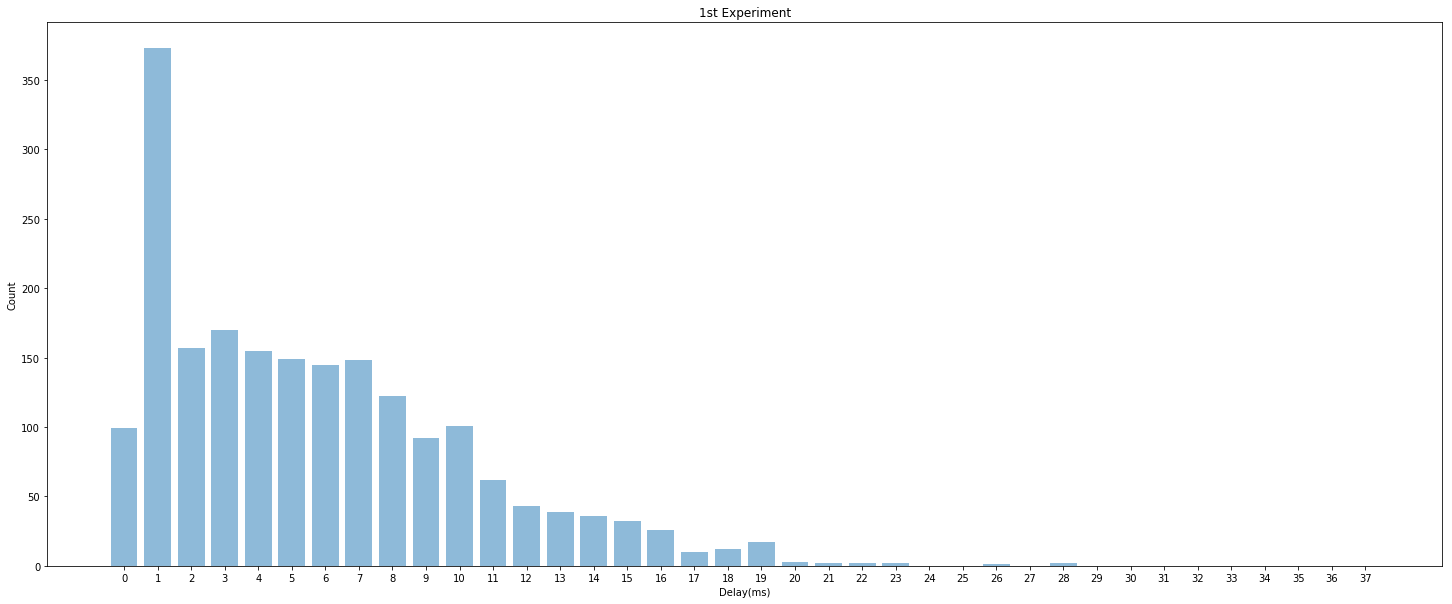
\includegraphics[width=9cm, height=4cm]{histogram_1.png}

\section{Setting Delays}
We calculated the end to end delay to extract the meaningful information from the network that we constructed. In order to do so, we needed to take some actions.
\subsection{Setting Local Times}
We first observed that the end to end delay times were negative or big positive numbers. We concluded that there must be some mistake for this to happen. So we set the local time of source node and destination node using following commands. \\
\texttt{sudo service ntp stop} \\
\texttt{sudo ntpdate -s time.nist.gov} \\
\texttt{sudo service ntp start} \\
After these commands, local times of the source and the destination node's machines were set the same. So, we could achieve the desired end to end delays properly.
\subsection{Setting Link Delays}
We needed to set the link delays in order to observe the given experiments. To do this, we put the delay on the left interface of the links. For example, to put a link delay from source to broker node, we needed to check the interface of left side of the link, the IP address is \texttt{10.10.1.1}. Then, using the \texttt{ifconfig} command we saw that port of this interface is \texttt{eth1}. So, using the following commands we were ready for the experiments. \\
\begin{itemize}
    \item Experiment 1: \\
    \texttt{sudo tc qdisc add dev eth1 root netem delay 1ms 5ms distribution normal}
    \item Experiment 2: \\
    \texttt{sudo tc qdisc add dev eth1 root netem delay 20ms 5ms distribution normal}
    \item Experiment 3: \\
    \texttt{sudo tc qdisc add dev eth1 root netem delay 60ms 5ms distribution normal}
\end{itemize}
The above command snippets are for first link only. We applied these to the other links as well with some configuration changes (i.e eth port changes).

\section{Experiment Observations}
As discussed above, we first implemented our network without acknowledgement. So we send whole packets at once and obtained the $packet number vs. time$ graph in Figure 1. We observed that after a certain packet number, end to end delays began increasing dramatically. Also there were some packet losses. When we analyze the reason for this, we saw that there was a bottleneck on our network. Although the bandwidth between the source and the broker node is 1000 kbytes per second, the bandwidth between other nodes are 10 kbytes per second. This situation resulted in bottleneck on the network. For this reason, we used acknowledgement to send the next packet and made the experiments accordingly. \\

\begin{figure}[t]
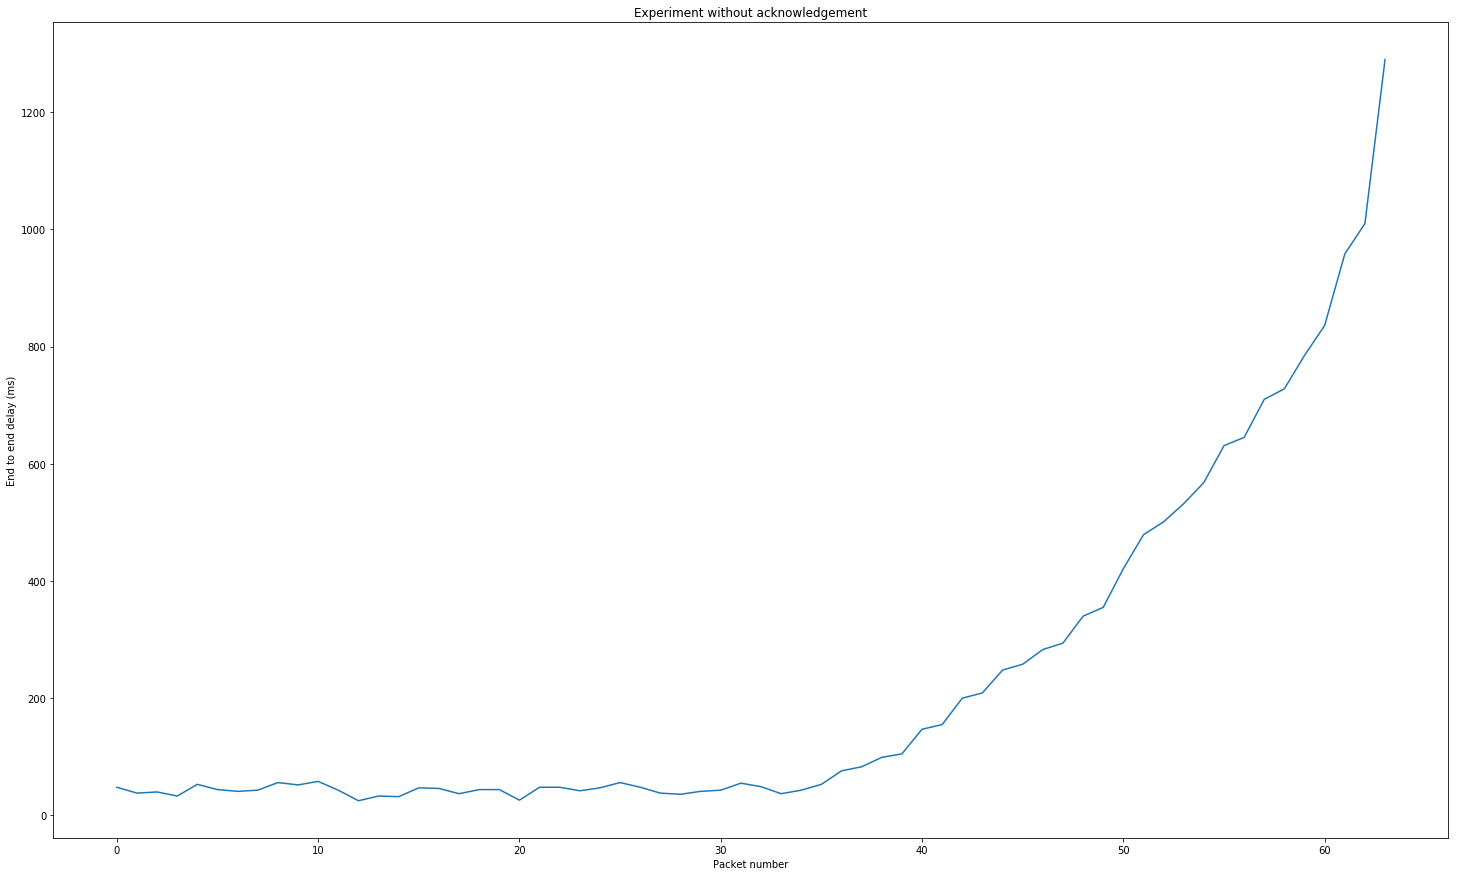
\includegraphics[width=8.5cm, height=7cm]{without_ack.png}
 \caption{Experiment Without Acknowledgement}
 \label{fig:1}
\end{figure}

When we tried without putting the delays on the network, we observed that end to end delays were 2-3ms on average. Then we set the delays on according to experiment. After setting the delays between nodes, we needed to see if the distribution of end to end times was normal or not. To do so, we created the frequency histograms to see the distributions. Define time of delay $d$ as a random variable and array of delays $ds$, following code snippet gives the histogram of the 1 experiment.\\
\texttt{for d in ds:} \\
\indent\texttt{histogram[d] += 1} \\

The bar chart in the Figure 2, Figure 3 and Figure 4 represent the histogram of the Experiment I, Experiment II and Experiment III respectively. All 3 charts were created using 2000 packets. All of the histograms are normal-like distributions and we can conclude from these diagrams that we were able to handle the end to end delays. In addition, we can conclude that the distribution in the Figure 1 is left-skewed normal distribution since it has a peak at value $1$ and the end to end delay for a packet can't be less than 0.

\begin{figure}[t]
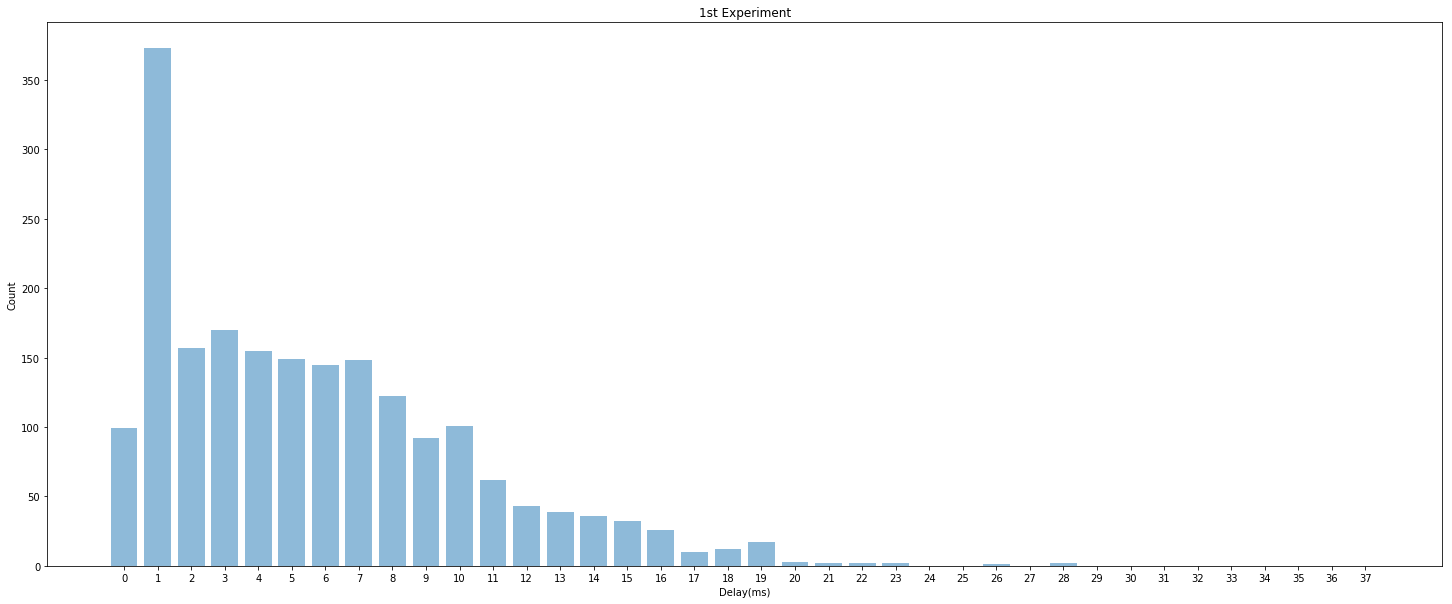
\includegraphics[width=8.5cm, height=7cm]{histogram_1.png}
 \caption{Experiment I Histogram}
 \label{fig:1}
\end{figure}

\begin{figure}[t]
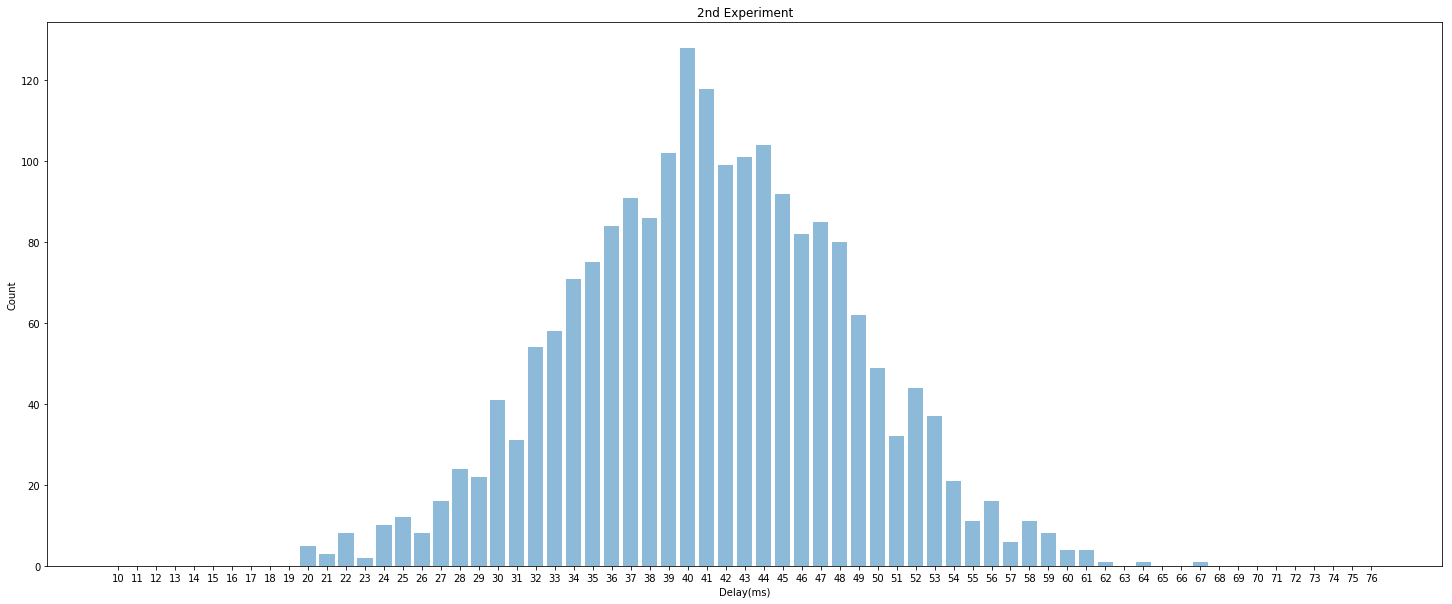
\includegraphics[width=8.5cm, height=7cm]{histogram_20.png}
 \caption{Experiment II Histogram}
 \label{fig:1}
\end{figure}

\begin{figure}[t]
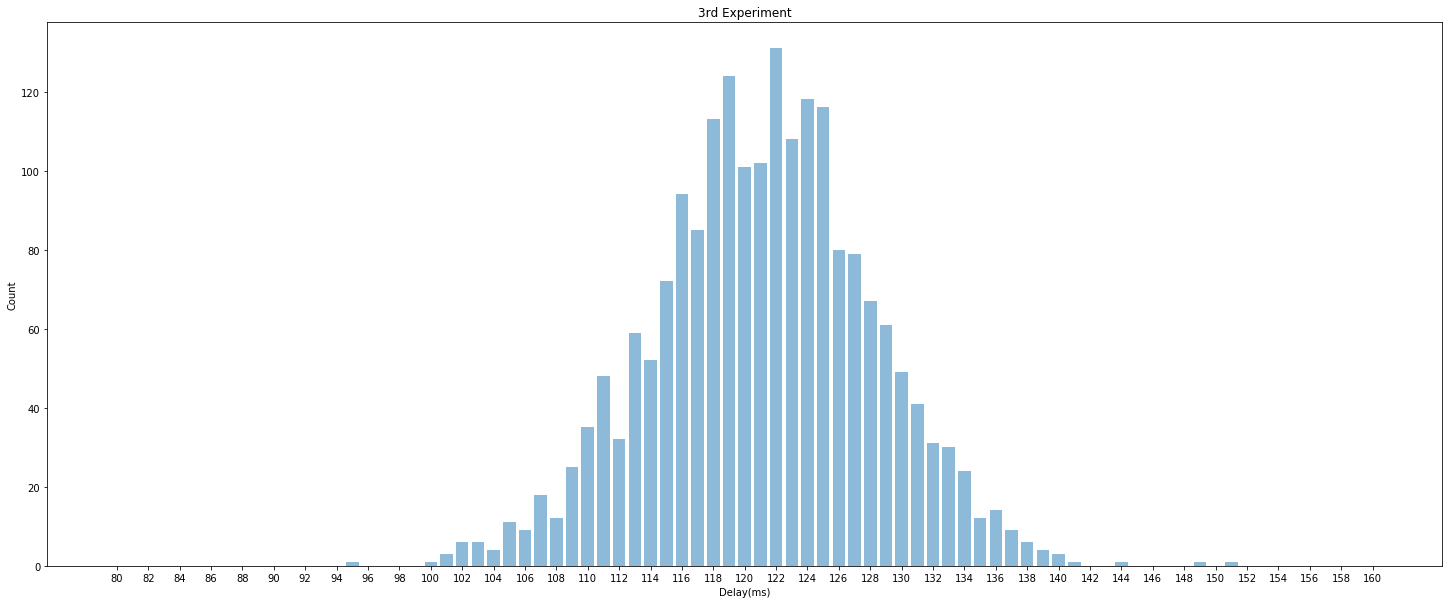
\includegraphics[width=8.5cm, height=7cm]{histogram_60.png}
 \caption{Experiment III Histogram}
 \label{fig:1}
\end{figure}

In Figure 5, we created a bar chart to give the reader an intuition about the relation between the Network Emulation Delay and End-to-End delay. We followed the following steps to calculate the information on the $cyan$ bars for each experiments.

\begin{itemize}
    \item We put end-to-end delays for each packets into an array \texttt{delays} of length $n=2000$. 
    \item We calculated the mean and the standard deviation (std) using \texttt{delays} array.
    \item In order to calculate the margin of error, we checked the $Z$-table for the $95\%$ confidence interval and obtained the result $z=1.96$.
    \item We calculated the margin of error using the equation 1.
    \begin{equation}
    error = \pm z \times \dfrac{std}{\sqrt{n}}\label{eq}
    \end{equation}
\end{itemize}

Using this margin of error, we plotted the Figure 4. In this figure, blue bars represent the network emulation delay given to us. Error bars represent margin of error, which is $\pm 15$. Also, cyan bars represent the mean of the end-to-end delays we calculated, error bars represent the margin of error, which $\pm error$ we obtained above. \\
We expect that mean of end-to-end delays will be close to the network emulation delay. Moreover, we expect that the error interval of the experiments will be between the error interval of the network emulation delay. We observed that their means are close to each other and the error interval of the experiments is between the error intervals of the network emulation delay. So, we were able to conclude that our experiments fit to the expected results.


\section{Conclusion}
To conclude, we constructed a network that handles the duties specified in the project description text. We first constructed our network without waiting acknowledgement and we saw that there were packet losses and the end to end delays were increasing as the number of packets increase due to differences between bandwidths of links. So, we waited for the acknowledgement to send the next packet. Using this, to see the distribution of the end to end delays, we obtained the charts in the figures 2, 3 and 4. We were required to make the distributions normal and as it can be seen from the graphs, we were able to do so using the $netem$ commands. Moreover, we plotted the Network Emulation Delay vs. End-to-End Delay in figure 5 and discussed the observations that can be made from this graphs, one of them is: we were required to fit our $mean\pm error$ values in between the intervals specified in the project description text.

\begin{figure}[t]
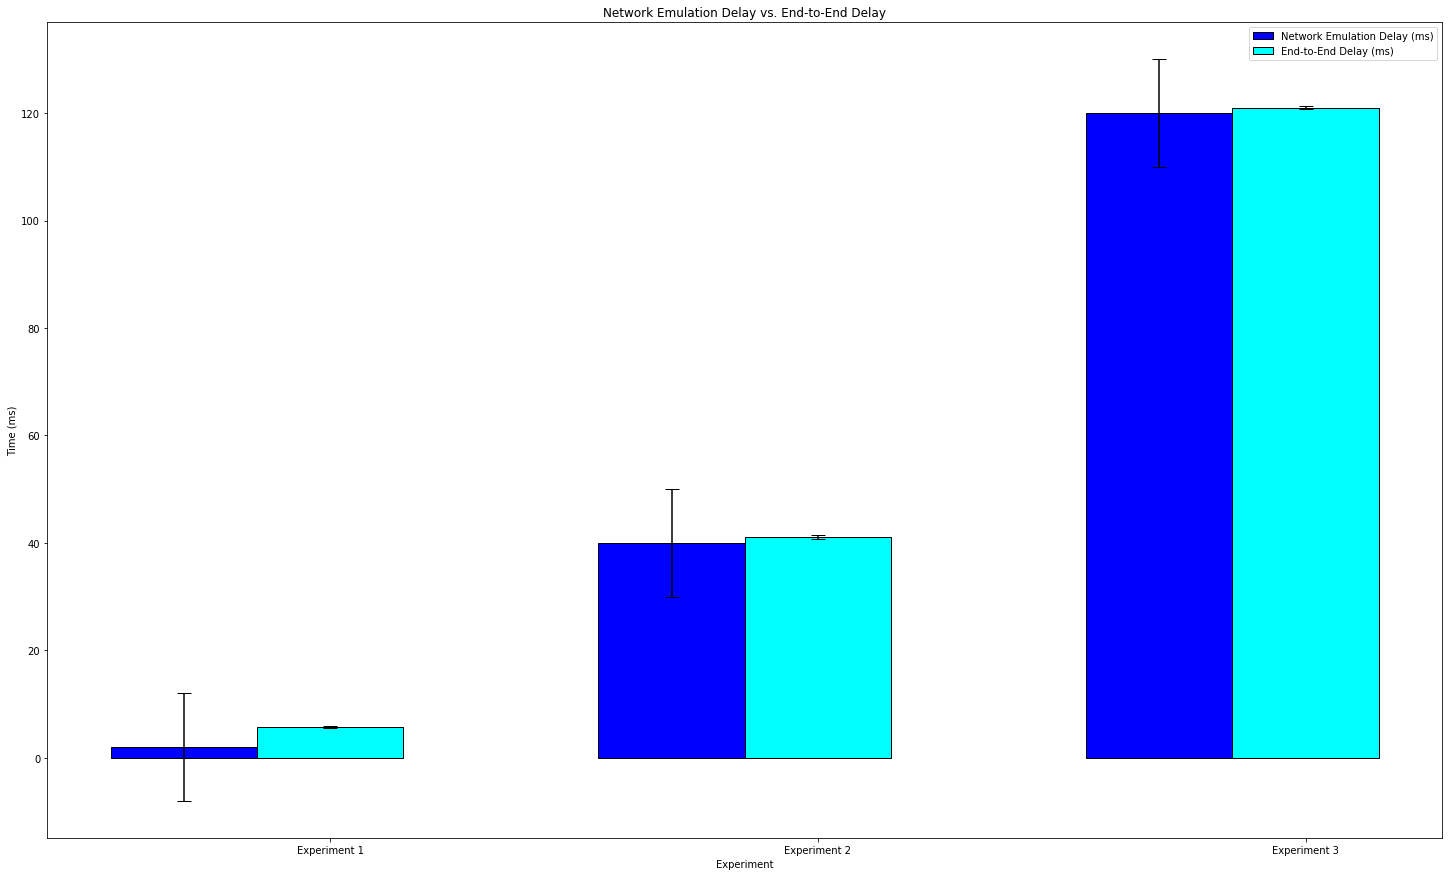
\includegraphics[width=8.5cm, height=7cm]{vs_graph.png}
 \caption{Network Emulation Delay vs. End-to-End Delay}
 \label{fig:1}
\end{figure}



\end{document}
